\documentclass[../TinyBot.tex]{subfiles}
\begin{document}

\section{Microcontroller} \label{sec:microcontroller}
\begin{wrapfigure}[4]{r}{0.3\textwidth}
    \vspace{-1cm}
    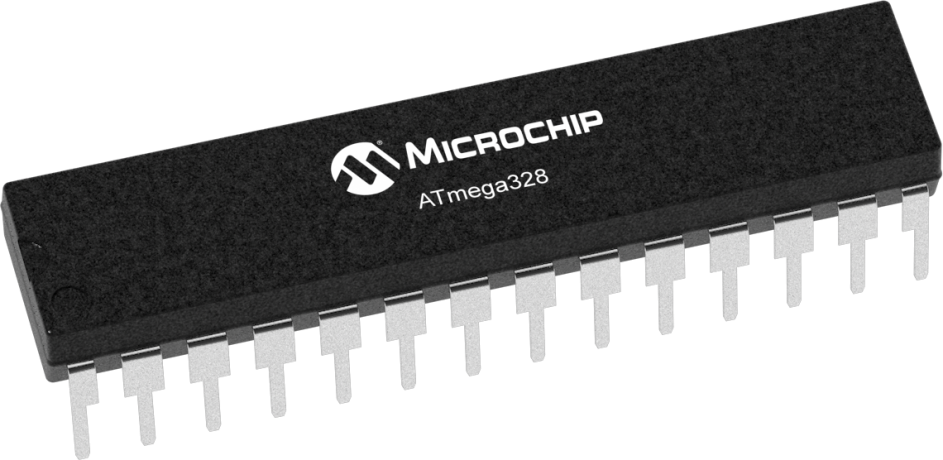
\includegraphics[width=0.25\textwidth]{medium-ATmega328-SPDIP-28.png}
    \captionof{figure}{A Microchip}
    \label{fig:microchip}
\end{wrapfigure}

A microcontroller is a really small microcomputer on a very small chip, see Figure \ref{fig:microchip}.
These are used in a variety of devices; including robots, vending machines, phones, computers, etc. \\

Arduino's are a development board; consisting of an microcontroller, power regulation, and input/output (also known as IO) pins. As microcontrollers are very tiny prototyping with them or using them to build something would be really difficult. The purpose of an arduino is to provide a medium that allows easy development with microcontrollers. There are many different kinds of arduinos, each using a different microchip. \\

\begin{wrapfigure}[10]{l}{0.35\textwidth}
    \centering
    \vspace{-0.5cm}
    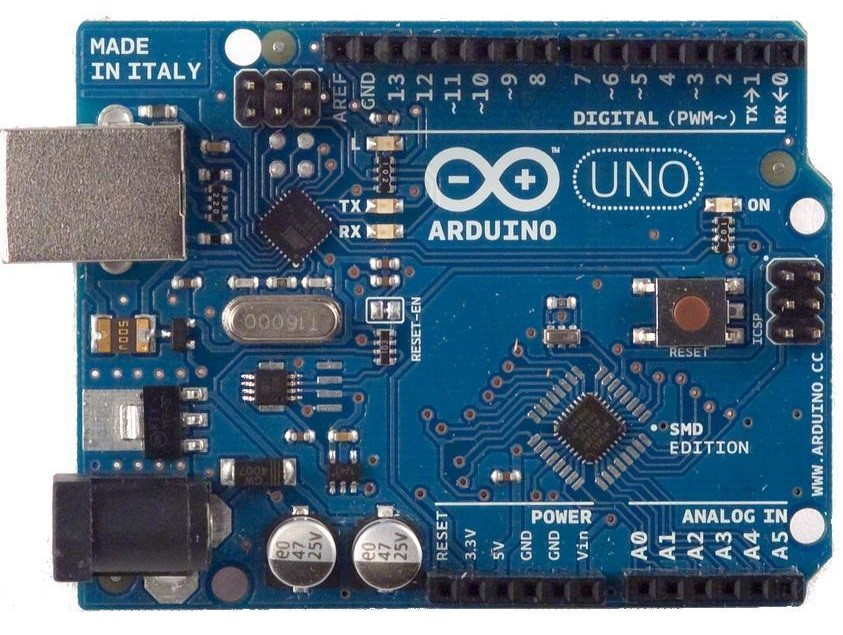
\includegraphics[width=0.33\textwidth]{arduino-uno.jpg}
    \caption{An Arduino Uno}
    \label{fig:arduino-real}
\end{wrapfigure}


% The Arduino used in this project is the Arduino Uno, which has an ATMega328p microchip as shown in Figure \ref{fig:microchip}. 
The difference between Arduino Uno, Mega, and Nano is the form factor and the microchip used on them. 
Figure \ref{fig:arduino-real} is what a real Arduino Uno looks like, though the colour and text may be different from brand to brand. Genuine Arduinos are quite expensive, there are many clones available which are much cheaper. Figure \ref{fig:arduino-pinout} shows a stylised view of an Uno, labelling all the different pinouts. \\

Arduino's and other development boards are used extensively by hobbyists, they are cheap, easy to use, and extremely versatile. Arduino's are used in nearly every CRoC project, and can be used in countless DIY projects. \\


An Uno has many different ports and pins. Figure \ref{fig:arduino-pinout} shows and labels all the different ports on a standard Uno. \\

An important distinction to make is between the pins 5V, 3.3V, and VIN. VIN stands for voltage in; and this port is used to supply power to the arduino from batteries. Power can also be supplied through the barrel jack connection, see the black rectangle like block on figure \ref{fig:arduino-pinout}. 

The 5V and 3.3V  pins supply 5 volts or 3.3 volts respectively for powering other commponents, such as LEDs, ICs, or sensors.  \\

\begin{warningbox}
    Never put supply voltage into the 3.3V or 5V pins; this will break the Arduino. 
\end{warningbox}


\begin{center}
    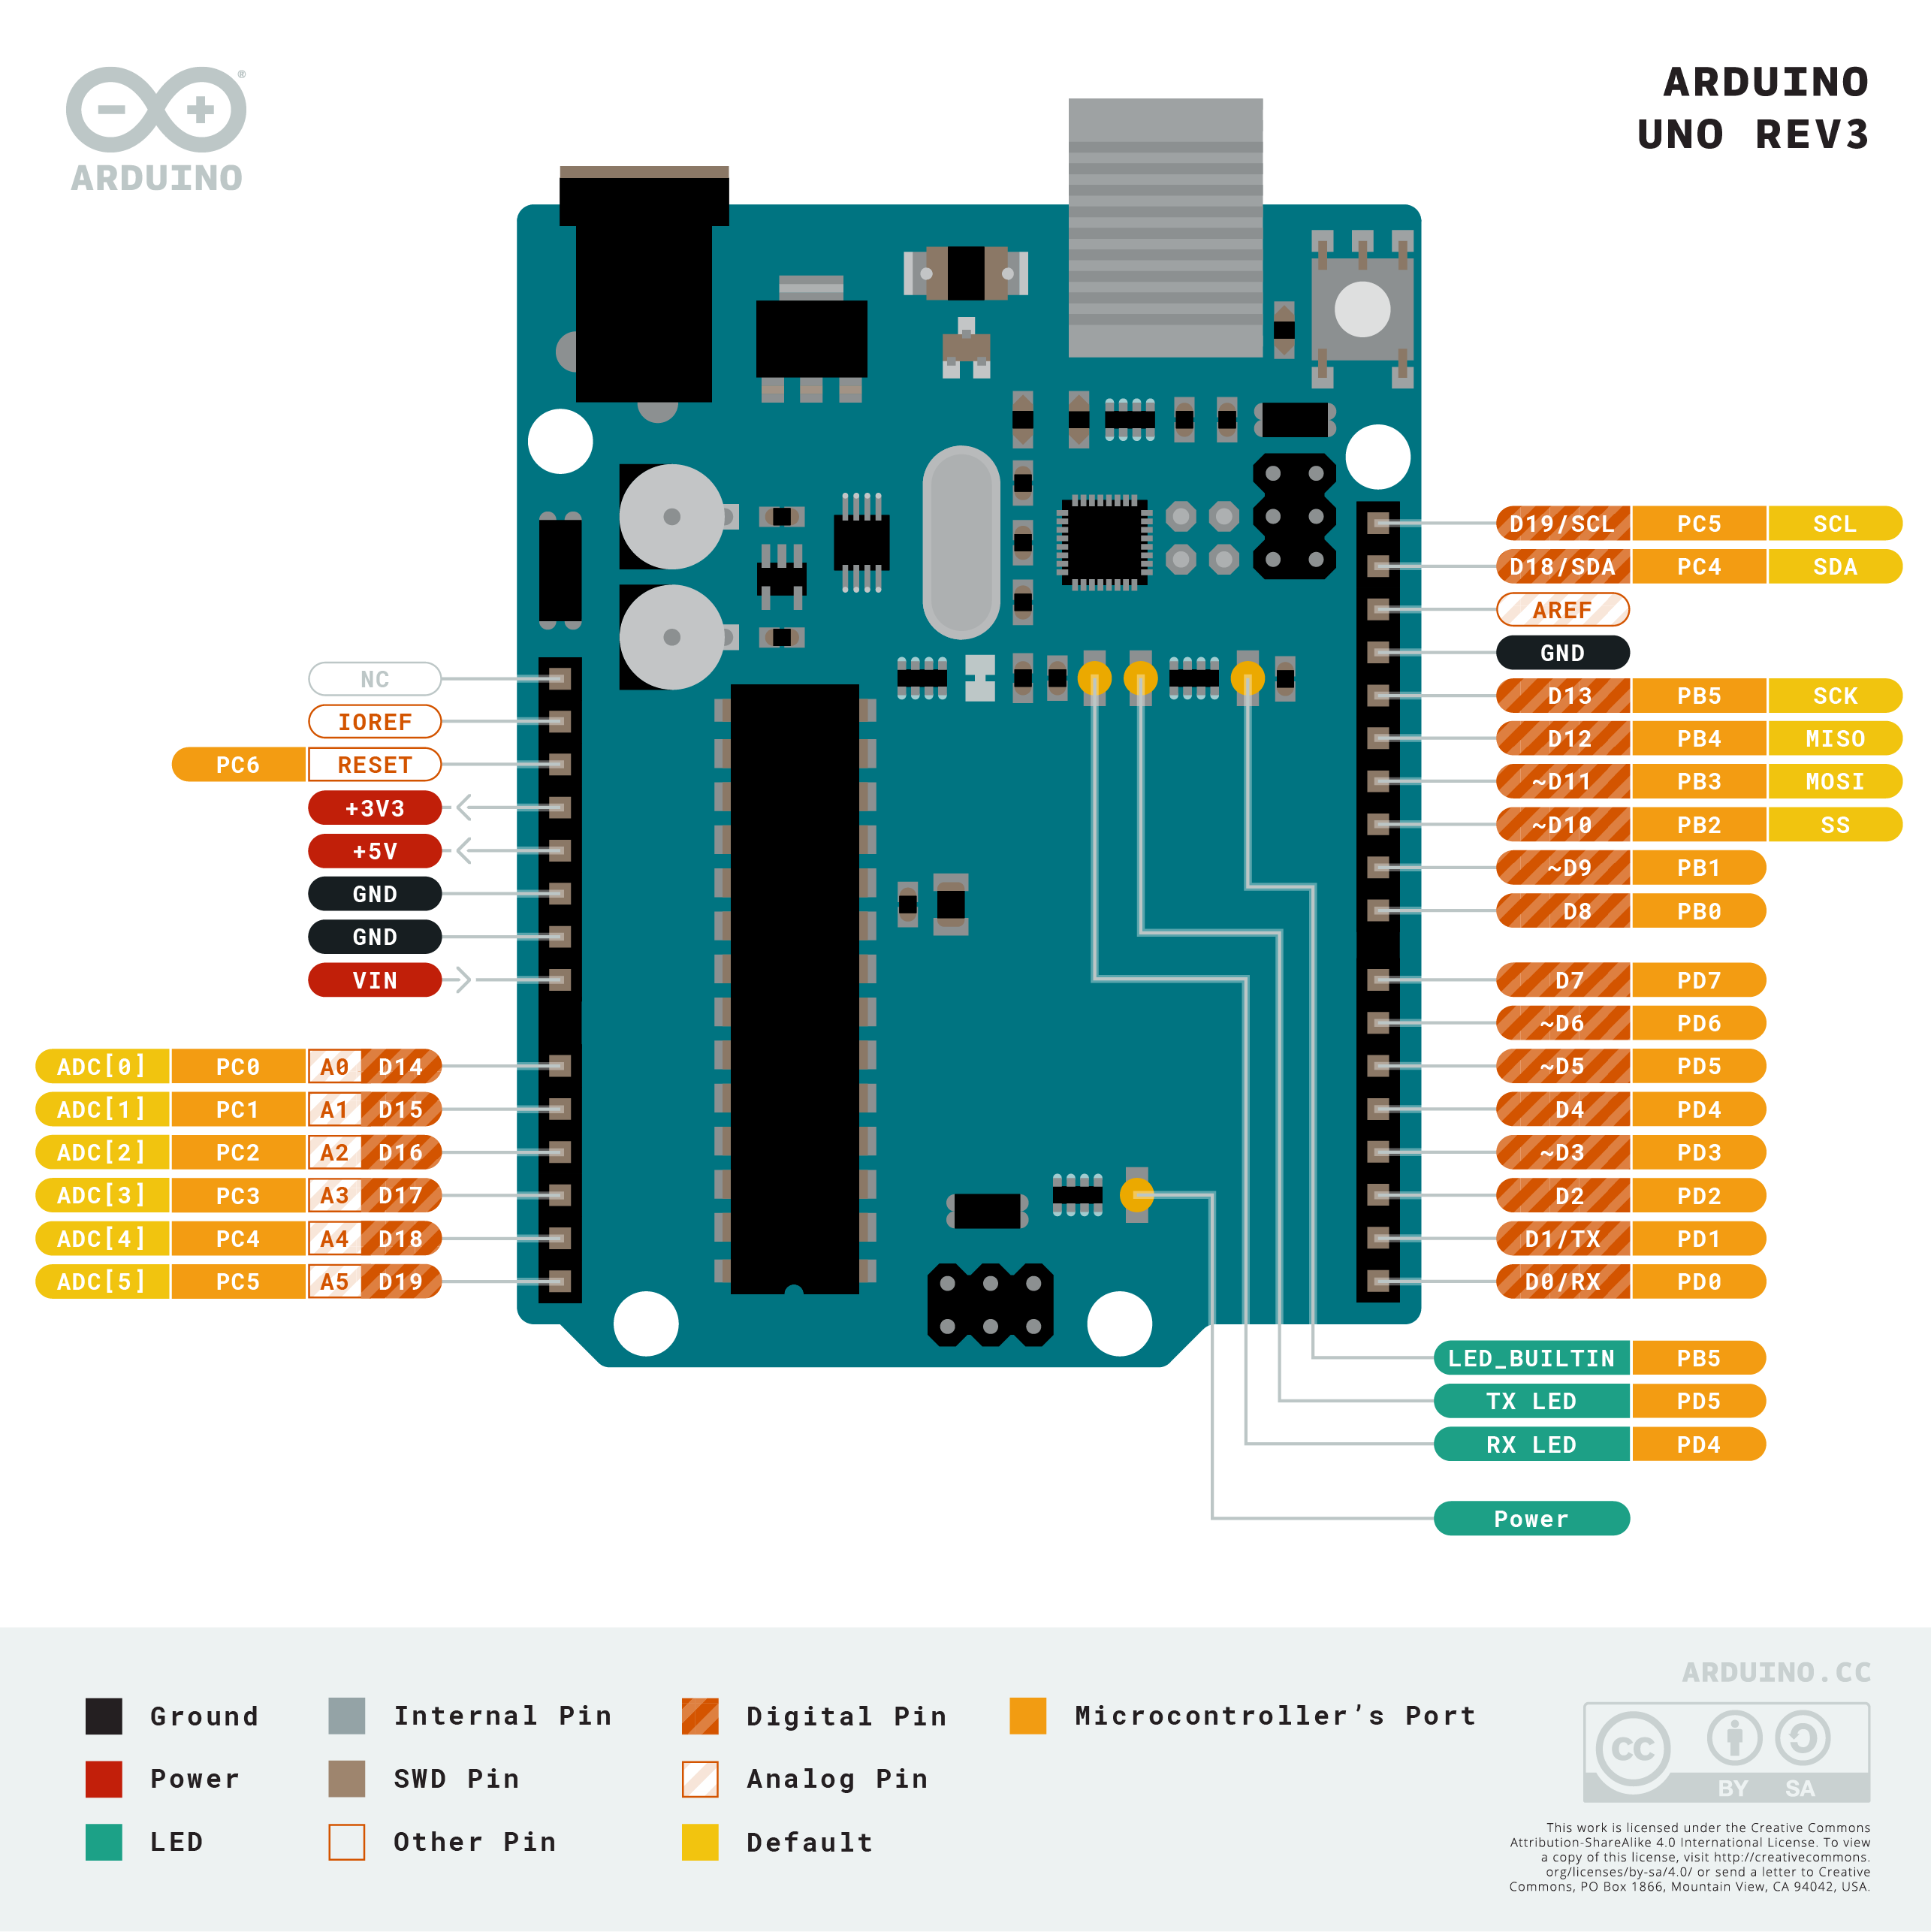
\includegraphics[width=\linewidth]{Pinout-UNOrev3_latest.png}
    \captionof{figure}{Pinout of Arduino Uno}
    \label{fig:arduino-pinout}
\end{center}


There are two different kinds of pins on an arduino, digital and analog. Look at the legend to see which pins are digital, The digital pin numbers all start with \lstinline[]!D!, just as the analog pins start with \lstinline[]!A!.
% (notice the pins on the right of the diagram labelled \lstinline[]!D0! to \lstinline[]!D13!) 
Analog pins can also be used as digital pins, but digital pins cannot be used as analog pins. \\


Digital pins can be set to \lstinline[]!HIGH! or \lstinline[]!LOW!, think of it like a button it can be on or off. Setting a pin to \lstinline[]!HIGH! turns it on, and \lstinline[]!LOW! turns it off. As circuits get more complicated, it is possible that setting a pin to \lstinline[]!LOW! will enable a part of the circuit; though for beginners it is best to think of \lstinline[]!HIGH! as on and \lstinline[]!LOW! as off; especially when working with a H-Bridge. 

% \$TODO - ANALOG PINS

\end{document}